\documentclass[10pt]{article}
\usepackage[a4paper,total={6in,8in}]{geometry}
%\usepackage{a4wide}
\usepackage{comment}
\usepackage{graphicx}
\usepackage{esint}    			 %package for integrals%
%\usepackage[utf8]{inputenc}
%\usepackage{attachfile}
\usepackage{layout}
%\usepackage{wrapfig}
\usepackage{listings}
\usepackage{url}
\usepackage{color}


%\graphicspath{ {/home/putlurhitheshreddy/Desktop/} }


\begin{document}
	
\begin{center}
	\textbf{\Large Assignment-8}\\
	\vspace{1mm}
	\textbf{\Large ELP-718 Telecom Software Laboratory}\\
	\textbf{Putlur Hithesh Reddy} \\
	\textbf{2018JTM2244} \\
	\textbf{2018-2020 }\\ 
	\textbf{A report presented for the assignment on \textbf{Python and github}} \\ [1.5 in]	
\end{center}

\begin{figure}[h!]
	\centering
	
\includegraphics{iitlogo} \\  [1.5 in]	
\end{figure}

\begin{center}
	\textbf{Bharti School of}\\ 
\textbf{Telecommunication Technology and Management }\\
\textbf{IIT DELHI}\\
\textbf{India}\\
\textbf{27-Sep-2018}
\end{center}

\newpage
\tableofcontents
\newpage

\section{\textbf{\Large Objective}}
 The assignment is designed to know about Python and the ease of programming in python. This also introduces to the basic usage of github and its relevance in software development life cycle
 
 
 
 
\section{\textbf{\large Problem Statement-1}}
\subsection{Problem Statement}
\textbf{ }
\begin{itemize}
		\item  
		\subitem 
		\item ​
		\item 
		\item 
		\item 
		\item 
		\item 
		\item 
\end{itemize}

\subsection{Algorithm and implementation}

\begin{itemize}
		\item 
		\item \cite{1} 	
		\item  
		\item 
		\item 
		\item 
\end{itemize}

\newpage

%\subsection{Flow-chart}
%\begin{figure}[h!]
%	\centering
%	\includegraphics[scale=0.6]{Screenshot3}
%\end{figure}

\subsection{Input and Output Format}
\begin{itemize}
		\item \textit{Input Format}
		\subitem awk -f ./ps1.awk CDR.txt 		
		\item \textit{Output Format}
		\subitem \cite{2}
		\subitem  
		\subitem 
		\subitem 
		\subitem 
\end{itemize}

\subsection{Test cases or Sample Inputs and Respective results}
\begin{itemize}
		\item \textit{Sample format}
		\subitem \textbf{MOC}
		\subitem 
\end{itemize}

\subsection{Difficulties faced}
\begin{itemize}
	\item 
	\item 
	\item
\end{itemize}

\newpage





\section{\textbf{\large Problem Statement-2}}
\subsection{Problem Statement}
\textbf{ }
\begin{itemize}
		\item  
		\item 
		\item 
		\item 
			
		
\end{itemize}

\subsection{Algorithm and implementation}
\begin{itemize}
		\item 
		\item  
		\item 
		\item 
		\item \cite{3}
\end{itemize}

\newpage

%\subsection{Flow-chart}
%\begin{figure}[h]
%	\centering
%	\includegraphics[scale=0.5]{Screenshot2}
%\end{figure}


\subsection{Input and Output Format}
\begin{itemize}
	\item \textit{Input Format}
	\subitem 
	\item \textit{Output Format}
	\subitem 
	\subitem 
	\subitem 
	\subitem 
	\subitem  
\end{itemize}

\subsection{Test cases or Sample Inputs and Respective results}
\begin{itemize}
	\item \textit{Sample format}
	\subitem \textbf{Number of input lines :20}
	\subitem 
	\subitem 
\end{itemize}

\subsection{Difficulties faced}
\begin{itemize}
	\item 
	\item 
	\item 
	\item
\end{itemize}

\newpage

\section{\textbf{\large C Programming Codes}}
%\lstinputlisting{ps1.awk}
%\lstinputlisting{ps2.awk}
%\begin{verbatim}
%\end{verbatim}

\section{\textbf{\large Screenshots related to coding}}
%\begin{figure}[h!]
%	\centering
%	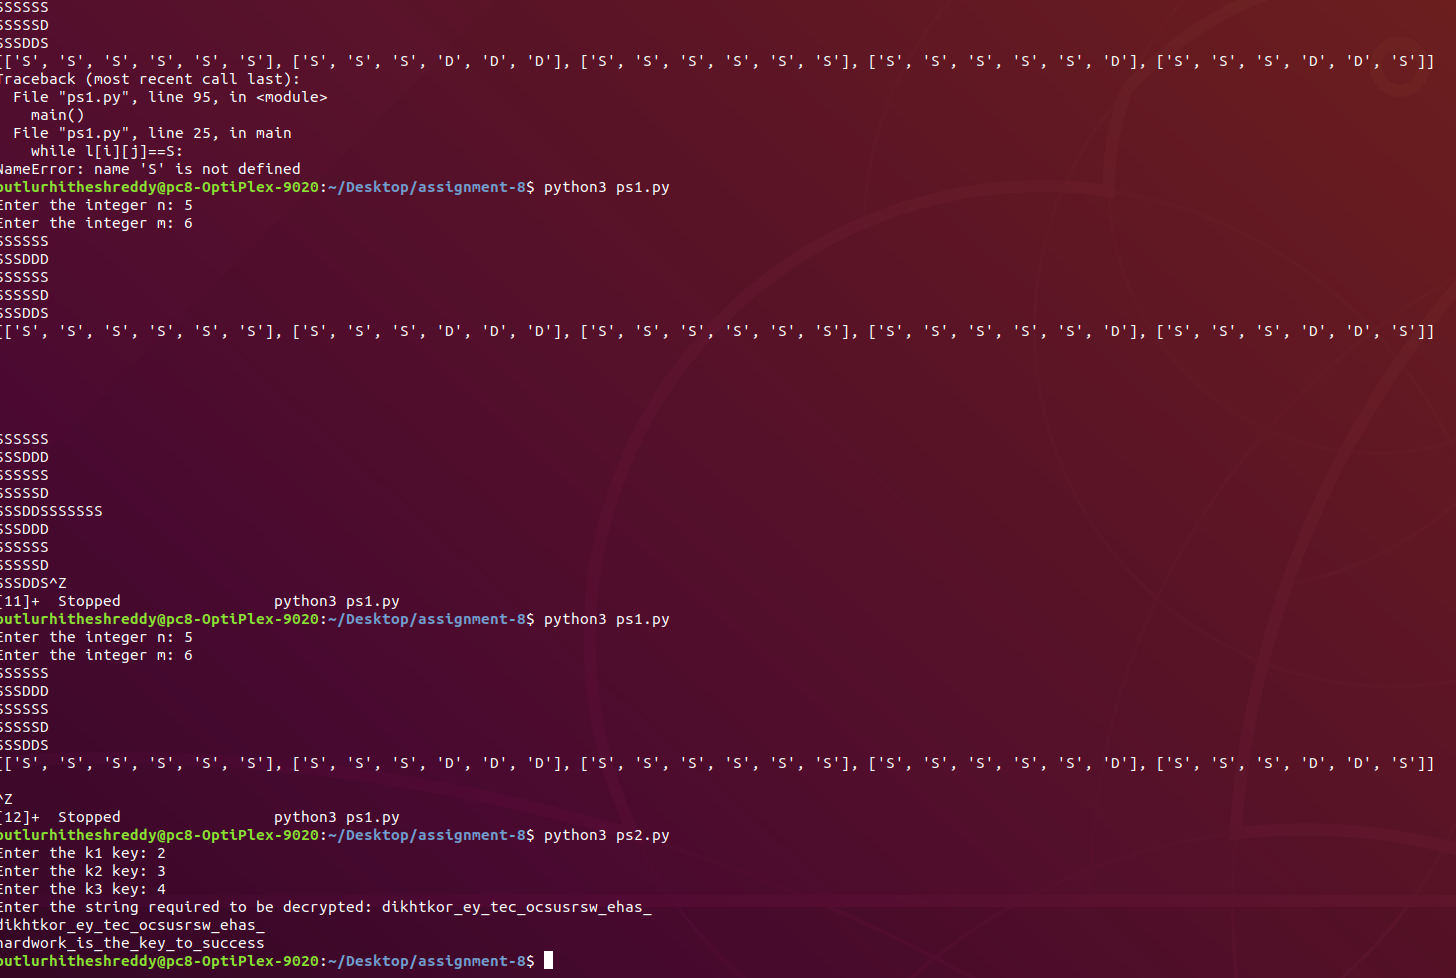
\includegraphics[width=15cm,height=8.5cm]{Screenshot1}
%\end{figure}
%\begin{figure}
%	\centering
%	\includegraphics[width=15cm,height=15cm]{Screenshot2}
%\end{figure}
%\begin{figure}
%	\centering
%	\includegraphics{Screenshot3}
%\end{figure}

\newpage

\bibliographystyle{plain} \bibliography{citations.bib}

\end{document}